% !TEX root = ../ejemplo-memoria.tex
% Contenidos del capítulo.
% Las secciones presentadas son orientativas y no representan
% necesariamente la organización que debe tener este capítulo.

% Diagramas de clases, de secuencia, de despliegue, diseño de
% pantallas, etc
\section{Diseño de base de datos}

La base de datos de la aplicación está diseñada para almacenar información sobre mujeres, sus lugares asociados, rutas temáticas, usuarios y el historial de visitas. El diseño sigue una estructura relacional y está implementado en \textbf{PostgreSQL} mediante modelos definidos en Django.

\subsection{Elección de la base de datos y justificación}

Se ha seleccionado \textbf{PostgreSQL} como sistema gestor de base de datos por su robustez, soporte avanzado de tipos de datos, integridad referencial y compatibilidad nativa con Django. PostgreSQL permite almacenar listas de valores en un solo campo, lo que resulta útil para atributos como las áreas de investigación asociadas a cada mujer, sin perder la capacidad de realizar consultas eficientes.

\subsection{Tablas principales y justificación de diseño}

A continuación se describen las tablas principales que conforman el modelo de datos, junto con la justificación de las decisiones tomadas:

\begin{itemize}
    \item \textbf{AreaInvestigacion}: Permite mantener un catálogo normalizado de áreas de investigación, facilitando la gestión y evitando duplicidades.
    \begin{itemize}
        \item \textbf{id} (clave primaria)
        \item \textbf{nombre}: nombre único del área.
    \end{itemize}
    \item \textbf{Mujer}: Representa a una mujer relevante. El campo \texttt{areas\_investigacion} se implementa como un \texttt{ArrayField} de cadenas, aprovechando las capacidades de PostgreSQL para almacenar múltiples áreas directamente en el registro, simplificando la consulta y el filtrado desde la API.
    \begin{itemize}
        \item \textbf{id} (clave primaria)
        \item \textbf{nombre}
        \item \textbf{descripcion}
        \item \textbf{foto}
        \item \textbf{areas\_investigacion}: lista de cadenas de texto (\texttt{ArrayField}) con los nombres de las áreas de investigación asociadas.
        \item \textbf{fechas}: información de fechas relevantes.
    \end{itemize}
    \item \textbf{Lugar}: Almacena información geolocalizada y la relación con una mujer. Se justifica la relación uno-a-muchos para poder asociar varios lugares a una misma mujer.
    \begin{itemize}
        \item \textbf{id} (clave primaria)
        \item \textbf{nombre}
        \item \textbf{descripcion}
        \item \textbf{latitud}
        \item \textbf{longitud}
        \item \textbf{foto}
        \item \textbf{ar\_url}: enlace a contenido de realidad aumentada.
        \item \textbf{mujer\_id} (clave foránea): referencia a la mujer destacada.
    \end{itemize}
    \item \textbf{Ruta}: Agrupa lugares y mujeres en recorridos temáticos. Se emplean relaciones ManyToMany para maximizar la flexibilidad y permitir que una ruta incluya múltiples mujeres y lugares, y viceversa.
    \begin{itemize}
        \item \textbf{id} (clave primaria)
        \item \textbf{nombre}
        \item \textbf{descripcion}
        \item Relación de tipo ManyToMany con las tablas \textbf{Mujer} y \textbf{Lugar}.
    \end{itemize}
    \item \textbf{UserProfile}: Extiende el modelo de usuario de Django para almacenar información adicional relevante para la aplicación, como la fecha de nacimiento.
    \begin{itemize}
        \item \textbf{id} (clave primaria)
        \item \textbf{user\_id} (relación uno a uno con User)
        \item \textbf{birth\_date}
        \item \textbf{email}
    \end{itemize}
    \item \textbf{VisitedLugar}: Permite registrar el historial de visitas de los usuarios a lugares concretos, facilitando la personalización y la obtención de estadísticas.
    \begin{itemize}
        \item \textbf{id} (clave primaria)
        \item \textbf{user\_id} (clave foránea)
        \item \textbf{lugar\_id} (clave foránea)
        \item \textbf{visited\_at}: fecha y hora de la visita.
    \end{itemize}
    \item \textbf{VisitedLugarRuta}: Permite registrar visitas de usuarios a lugares dentro de rutas específicas, lo que posibilita analizar el recorrido de los usuarios y mejorar la experiencia de gamificación.
    \begin{itemize}
        \item \textbf{id} (clave primaria)
        \item \textbf{user\_id} (clave foránea)
        \item \textbf{ruta\_id} (clave foránea)
        \item \textbf{lugar\_id} (clave foránea)
        \item \textbf{visited\_at}: fecha y hora de la visita.
    \end{itemize}
\end{itemize}

\subsection{Relaciones entre tablas}

\begin{itemize}
    \item Un \textbf{Lugar} pertenece a una \textbf{Mujer} (relación uno a muchos).
    \item Una \textbf{Mujer} puede tener varios \textbf{Lugares} asociados.
    \item Una \textbf{Ruta} puede incluir varias \textbf{Mujeres} y varios \textbf{Lugares} (relaciones ManyToMany).
    \item Un \textbf{UserProfile} extiende a un \textbf{User} de Django (relación uno a uno).
    \item \textbf{VisitedLugar} y \textbf{VisitedLugarRuta} permiten registrar el historial de visitas de los usuarios, tanto de lugares individuales como de lugares dentro de rutas.
\end{itemize}

\subsection{Esquema de tablas}

El siguiente esquema resume la estructura de las tablas principales de la base de datos. Para mejorar la visualización y evitar cortes de línea, se utiliza el entorno \texttt{tabularx}:

\begin{table}[H]
\centering
\begin{tabularx}{\textwidth}{l X}
\textbf{Tabla} & \textbf{Campos principales} \\
\hline
Mujer & id, nombre, descripcion, foto, areas\_investigacion (ArrayField), fechas \\
Lugar & id, nombre, descripcion, latitud, longitud, foto, ar\_url, mujer\_id (FK) \\
Ruta & id, nombre, descripcion, mujeres (M2M), lugares (M2M) \\
UserProfile & id, user\_id (O2O), birth\_date, email \\
VisitedLugar & id, user\_id (FK), lugar\_id (FK), visited\_at \\
VisitedLugarRuta & id, user\_id (FK), ruta\_id (FK), lugar\_id (FK), visited\_at \\
AreaInvestigacion & id, nombre \\
\end{tabularx}
\caption{Esquema resumido de las tablas principales de la base de datos}
\end{table}

\subsection{Justificación global del diseño}

El modelo de datos relacional implementado garantiza la integridad y la eficiencia en las consultas. El uso de \texttt{ArrayField} en \textbf{Mujer} permite una mayor flexibilidad y rendimiento en la consulta de áreas de investigación, sin necesidad de realizar joins adicionales, lo que es especialmente útil para filtros rápidos en la API. Las tablas de historial de visitas están separadas para facilitar la obtención de estadísticas, la personalización de la experiencia del usuario y la escalabilidad futura (por ejemplo, para añadir logros o recomendaciones personalizadas).
\begin{landscape}
    \begin{figure}
        \centering
        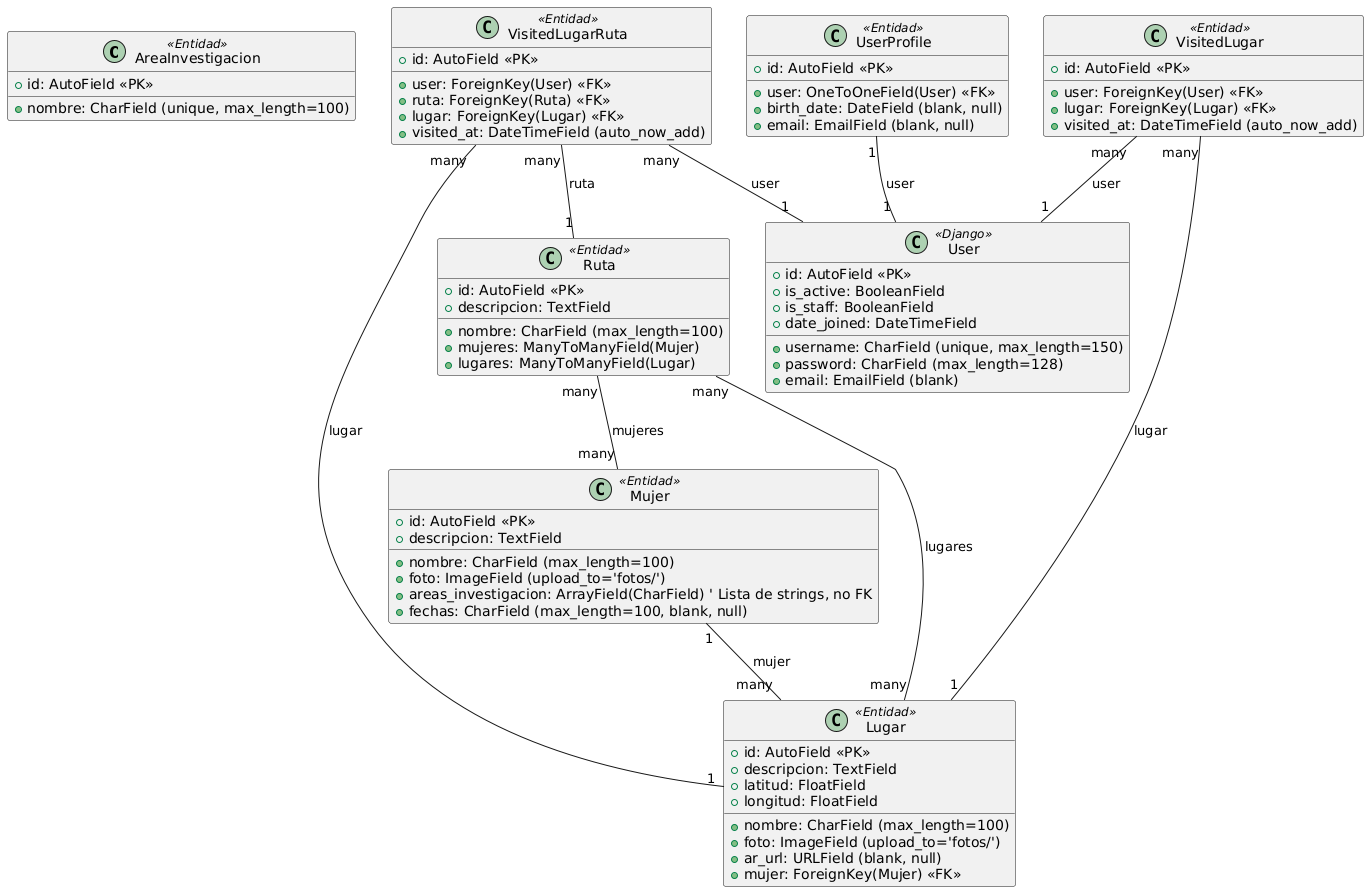
\includegraphics[width=1.2\paperwidth]{figs/diagrama_clases.png}
        \caption{Diagrama de clases de la base de datos}
    \end{figure}
\end{landscape}
\section{Diseño de la arquitectura del frontend}

El frontend de la aplicación está desarrollado en \textbf{React Native}, siguiendo una arquitectura basada en componentes funcionales y el uso de contextos para la gestión eficiente del estado global.El hecho de que el diseño sea modular y esté desacoplado hace que sea más sencillo de mantener y escalar, además de permitir añadir nuevas funcionalidades sin complicaciones. Esto también ayuda a que la experiencia de usuario sea más fácil de adaptar en un futuro con nuevas necesidades.

\subsection{Diagrama de clases del frontend}

La Figura~\ref{fig:clases-frontend} muestra el diagrama de clases que representa la arquitectura principal del frontend. Los componentes se agrupan en paquetes según su responsabilidad funcional: contextos, navegación, usuario, rutas, lugares y utilidades.

\begin{itemize} \item \textbf{Contextos:} El componente \texttt{FiltrosContext} centraliza la gestión del estado global de los filtros aplicados en la aplicación, proporcionando métodos para su actualización y reseteo. Este contexto es consumido por componentes como \texttt{Filtros}, \texttt{Rutas} y \texttt{Mapa}, permitiendo la sincronización de los criterios de filtrado en toda la interfaz. \item \textbf{Navegación:} El componente \texttt{NavigationApp} implementa la navegación principal mediante un \textit{stack navigator}, gestionando el flujo entre pantallas y facilitando la transición entre las distintas funcionalidades de la app. \item \textbf{Componentes de Usuario:} Incluyen las pantallas de autenticación (\texttt{Login}, \texttt{Register}), el perfil de usuario (\texttt{PerfilUsuario}) y el acceso al historial de lugares y rutas visitadas (\texttt{HistorialLugares}, \texttt{HistorialRutas}). Cada uno de estos componentes gestiona su propio estado y lógica de interacción, garantizando la personalización y seguridad de la experiencia de usuario. \item \textbf{Componentes de Rutas y Lugares:} \texttt{Rutas} y \texttt{Mapa} permiten al usuario explorar rutas temáticas y lugares geolocalizados, respectivamente. Los componentes \texttt{Detail}, \texttt{HistorialLugares} y \texttt{HistorialRutas} permiten consultar información detallada de los lugares y el registro de visitas de estos, integrando la lógica de interacción con el backend. \item \textbf{Componentes de Utilidad:} Incluyen \texttt{Filtros}, \texttt{Mujeres} (visualización combinada de mujeres y lugares), la pantalla de bienvenida (\texttt{Welcome}), la lógica de realidad aumentada (\texttt{AR}), y la lógica de notificaciones de proximidad (\texttt{NotificacionProximidad}), que se ejecuta de forma invisible para el usuario y activa notificaciones según la localización. \end{itemize}

Las relaciones entre componentes reflejan tanto el consumo de contexto (\textit{consume}), como la navegación entre pantallas (\textit{navega a}), y el uso de lógica auxiliar (por ejemplo, la integración de notificaciones en el componente principal \texttt{Main}).

\begin{landscape} \vfill \begin{figure}[H] \centering 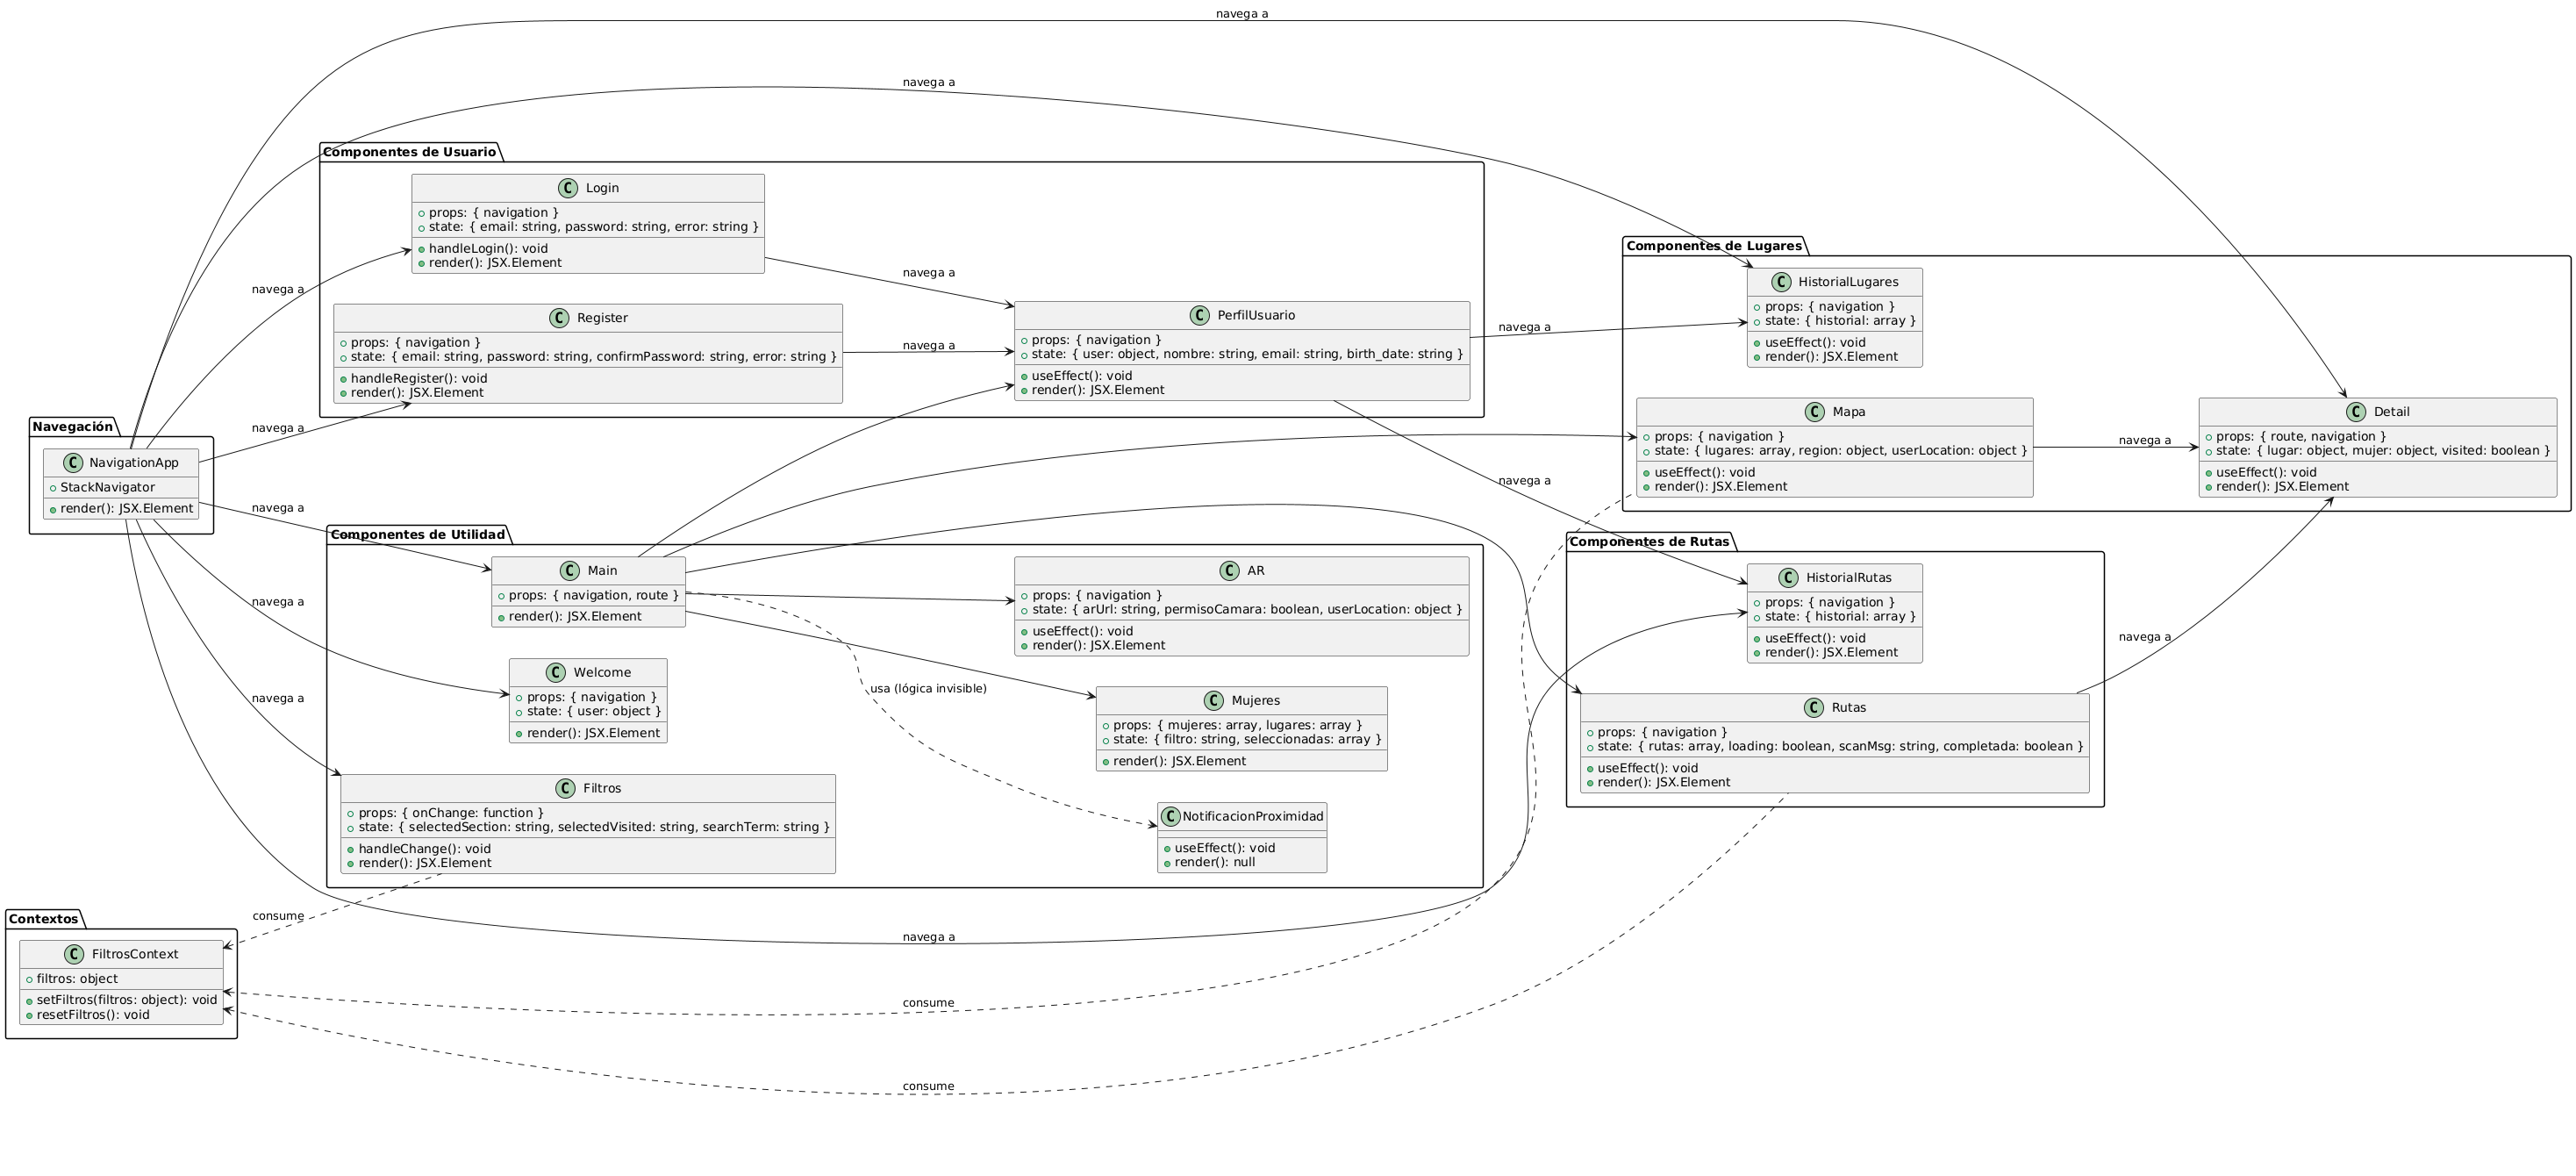
\includegraphics[width=1.2\paperwidth]{figs/prueba.png} \caption{Diagrama de clases del frontend React Native: estructura de componentes y relaciones principales.} \label{fig:clases-frontend} \end{figure} \vfill \end{landscape}